\section{Part 3: Display for control and overview of the process}

This section gives an overview of the modules used in the project. As shown in Figure \ref{motor_fp} a library was created containing control modules for the Generator, Heater and Motor 


\subsection{Motor Faceplate}
From Figure \ref{motor_fp} information about the motor status, running (green), stopped (red), ready (yellow) is given. The speed can be manually controlled. As well to reading the actual output from the IO modules, and the calculated RPM value.
\begin{figure}[!htb]
    \centering
    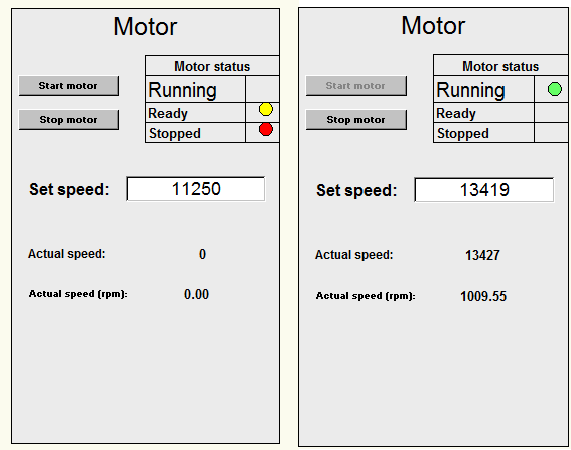
\includegraphics[scale=0.7]{images/Motor_Status}
    \caption{Motor Faceplate}
    \label{motor_fp}

\end{figure}

\begin{figure}[!htb]
    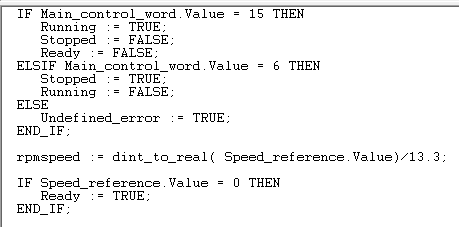
\includegraphics[scale=0.8]{images/motor_ST}
    \caption{Motor Structured Text}
    \label{motor_st}

\end{figure}

\subsection{Generator Faceplate}

Figure \ref{Generator_fp} shows the faceplate for the generator, this gives information about the power consumption of the load, as well to connecting/disconnecting the load.

\begin{figure}[!htb]
    \centerline{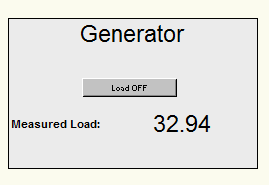
\includegraphics[scale=1]{images/Generator}}
    \caption{Generator Faceplate}
    \label{Generator_fp}

\end{figure}

\hfill \break

\subsection{Heater Faceplate}

Figure \ref{HeaterFaceplate} shows the heaters faceplate, which gives the the current temperature value (under the slope), the states of both pressure and temperature (on/off).

\begin{figure}[!htb]
    \centerline{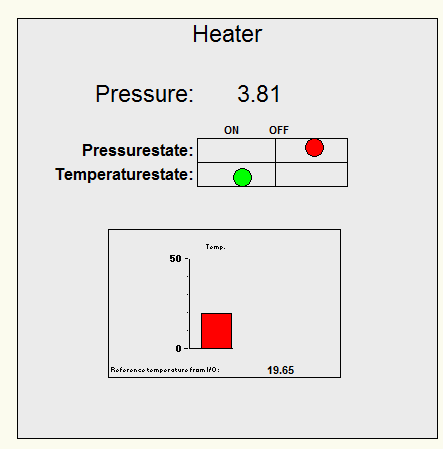
\includegraphics[scale=0.7]{images/Pressure_state_off}}
    \caption{Heater Faceplate}
    \label{HeaterFaceplate}

\end{figure}


\subsection{Overview of the Process}
A human interface of the motor, generator, heater and temperature regulator is shown in Figure \ref{Overview2}. While Figure \ref{Overview} shows the structure of the program.

\begin{figure}[!htb]
    \centerline{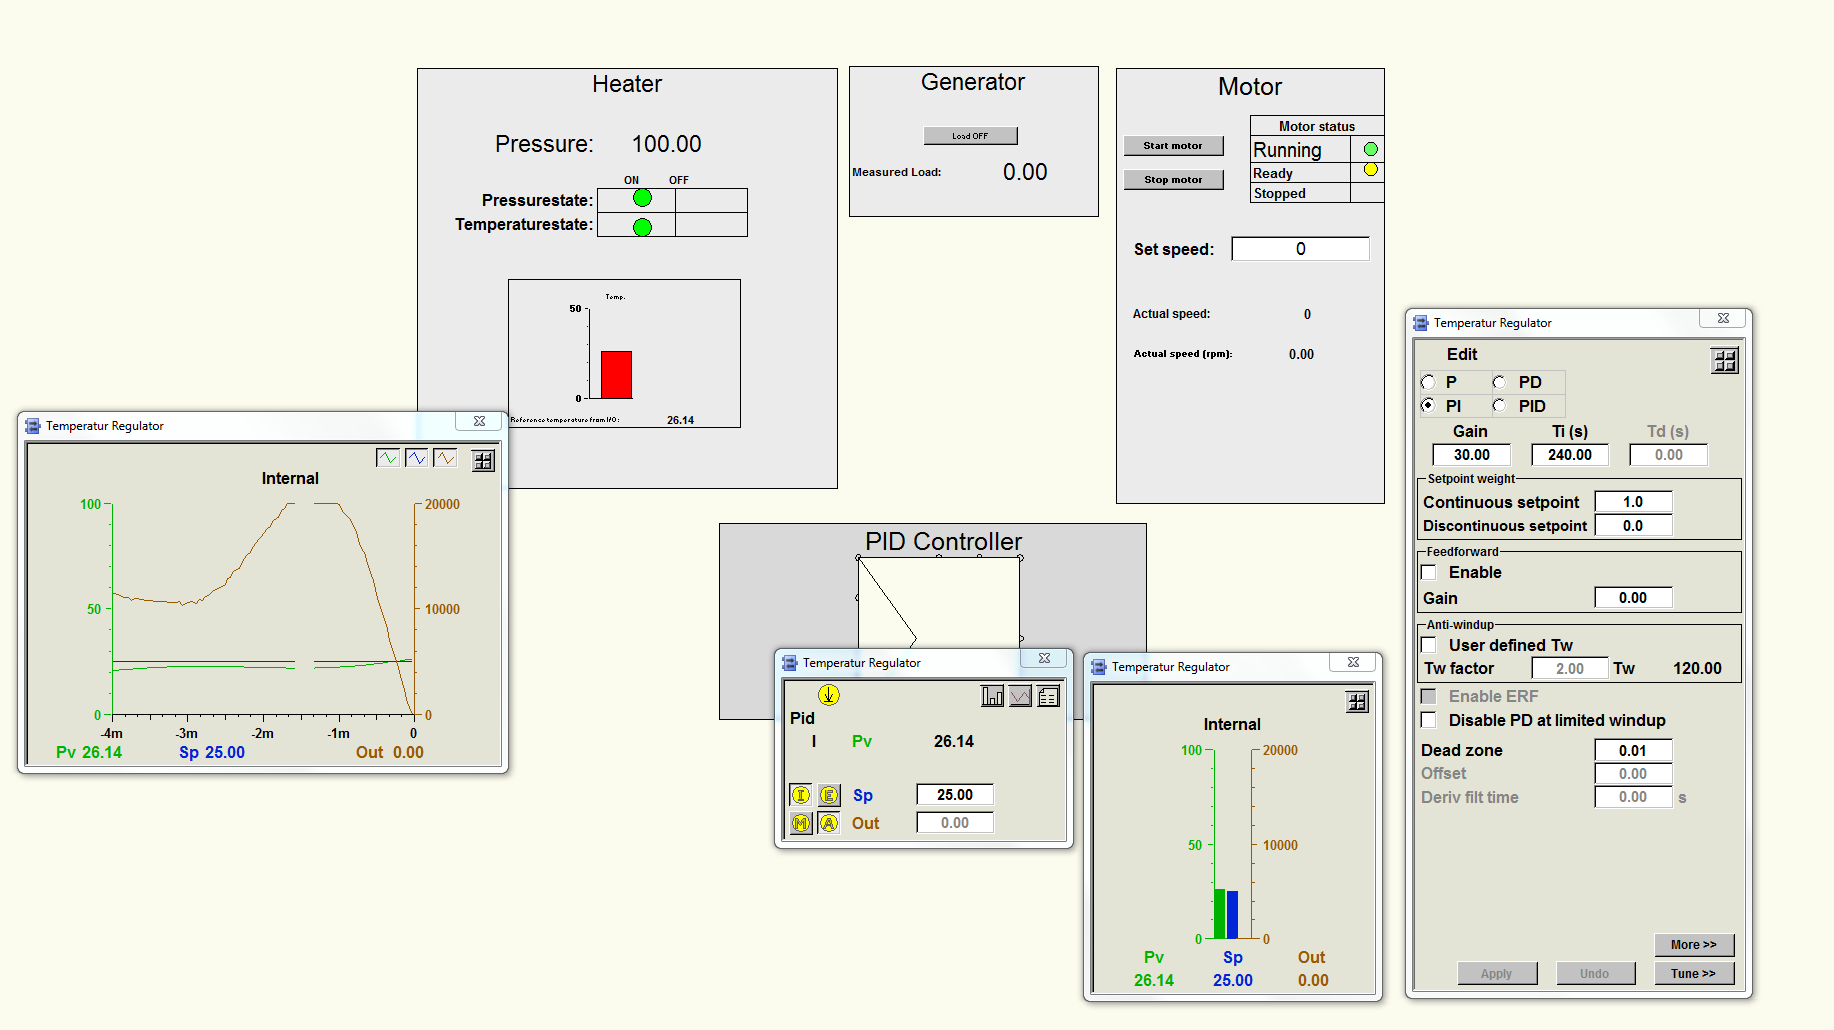
\includegraphics[scale=0.35]{images/overview2}}
    \caption{Overview HMI}
    \label{Overview2}
\end{figure}


\begin{figure}[!htb]
    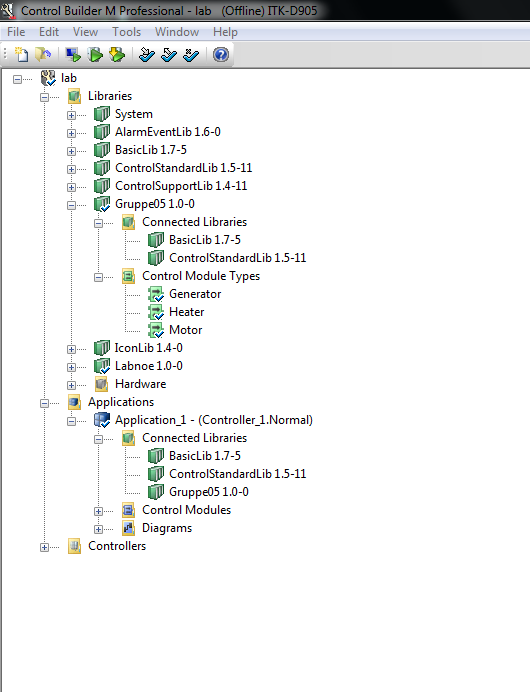
\includegraphics[scale=0.7]{images/overview}
    \caption{Overview structure}
    \label{Overview}
\end{figure}


